\let\oldvec\vec % Store \vec in \oldvec
\documentclass{llncs}
\let\vec\oldvec % Restore \vec from \oldvec

\usepackage[utf8]{inputenc}
\usepackage{url}
\usepackage{cite}
\usepackage{hyperref}
\usepackage{graphicx}
\usepackage{acronym}
\usepackage{float}
\usepackage{pgfgantt}
\usepackage{fixltx2e}
\usepackage{mathtools}
\usepackage{amsmath}
\usepackage{booktabs}
\usepackage{array}
\usepackage{subcaption}

%% REDUCE TEXT SIZE
% \addtolength{\textwidth}{1cm}
% \addtolength{\textheight}{1cm}

%% change bullet style
\renewcommand{\labelitemi}{$\bullet$}

\begin{document}

\title{Happiness in the United States: Measuring the Sentiment of Geolocated Tweets}

\author{João Ferreira Loff \newline \email{joao.loff@tecnico.ulisboa.pt}}
\institute{Universidade de Lisboa - Instituto Superior Técnico}

\maketitle

\begin{abstract}
DO QUE FALAR NO ABSTRACT?
\end{abstract}


\section{Introduction}

FAZER UM RESUMO DO RESTO DO PAPER? MOSTRAR JÁ RESULTADOS/CONCLUSÕES?

We structure our paper as follows. In Section II, we describe the data sets. In Section III we describe our methodology for measuring happiness. In Section IV we measure the happiness of different states and cities and determine the happiest and saddest states in the US, and at the same time we compare our results with the Gallup-Healthways Well-being Index \cite{GallupHealthway2013}. We conclude with a discussion and a reference for future work in Section IV.

\section{Related Work}

In \cite{Mitchell2013,Dodds2011,Frank2013} the overall aim is to investigate how geographic place correlates with and potentially influences societal levels of happiness. In particular they ask if it is possible to (a) measure the overall average happiness of people located in US states and cities, and (b) explain the variation in happiness across different states and cities.
The first question is answered using word frequency distributions collected from a large corpus of \emph{tweets} posted on Twitter, with individual words scored for their happiness using the technique by Dodds et al. \cite{Dodds2009}, which is an improvement of the original ANEW approach \cite{Bradley1999}. To answer the second question of happiness variability, they examine how individual word usage correlates with happiness and various social and economic factors, using the ‘word shift graph' technique developed in \cite{Dodds2011,Dodds2009}, and socioeconomic census data to attempt to explain the usage of certain words.
To obtain a score for a given tweet T containing N unique words, they calculate the average happiness $h_{avg}$ using an weighted average of the number of times a word occurs in T, multiplied by the the $h_{avg}$ of that specific word. In the end we dived that weighted average of all the words, with the total number of detected LabMT words. Finally they used the average of the scores, to achieve the happiness scoring of a given state.

In \cite{Schwartz2013} FALAR DESTE

In \cite{Bertrand2013} FALAR DESTE

In \cite{Connor2010} FALAR DESTE


\section{Datasets}
\label{sec:datasets}

We examine a corpus of over 232 million tweets gathered from all over the world during the calendar year of 2012 \footnote{available at http://dmir.inesc-id.pt/shinra/~bmartins/twitter-data/data/}. After an initial parsing effort, we reduced the data set to have only geotagged tweets, which is near 0.78\% of the whole data set (less than 1.8 million tweets). For the present study, we focus only on the geotagged tweets located in the Continental United States (we excluded Alaska and Hawaii), which is near 27\% of the geotagged tweets (less than 0.5 million tweets).

State areas are defined using the \emph{state} data set available in the R \emph{maps} package \footnote{available at http://cran.r-project.org/web/packages/maps/}.

To measure sentiment (hereafter happiness) in these areas from the corpus of words collected, we use the Language Assessment by Mechanical Turk (LabMT) word list (available online in the supplementary material of \cite{Dodds2011}), assembled by combining the 5'000 most frequently occurring words in each of four text sources: Google Books (English), music lyrics, the New York Times and Twitter. A total of roughly 10'000 of these individual words have been scored by users of Amazon’s Mechanical Turk service on a scale of 1 (sad) to 9 (happy), resulting in a measure of average happiness for each given word \cite{Kloumann2012}. For example, ‘rainbow’ is one of the happiest words in the list with a score of $h_{avg}$ = 8.1, while ‘earthquake’ is one of the saddest, with $h_{avg}$ = 1.9. Neutral words like ‘the’ or ‘thereof’ tend to score in the middle of the scale, with $h_{avg}$ = 4.98 and 5 respectively.

Fig. \ref{fig:tweets_by_state} have the numbers per state of: the number of total tweets, the number of tweets that have LabMT words, and finally the percentage of the tweets that have LabMT words relatively to the total number. In median we have

\begin{figure}[!ht]
\centering
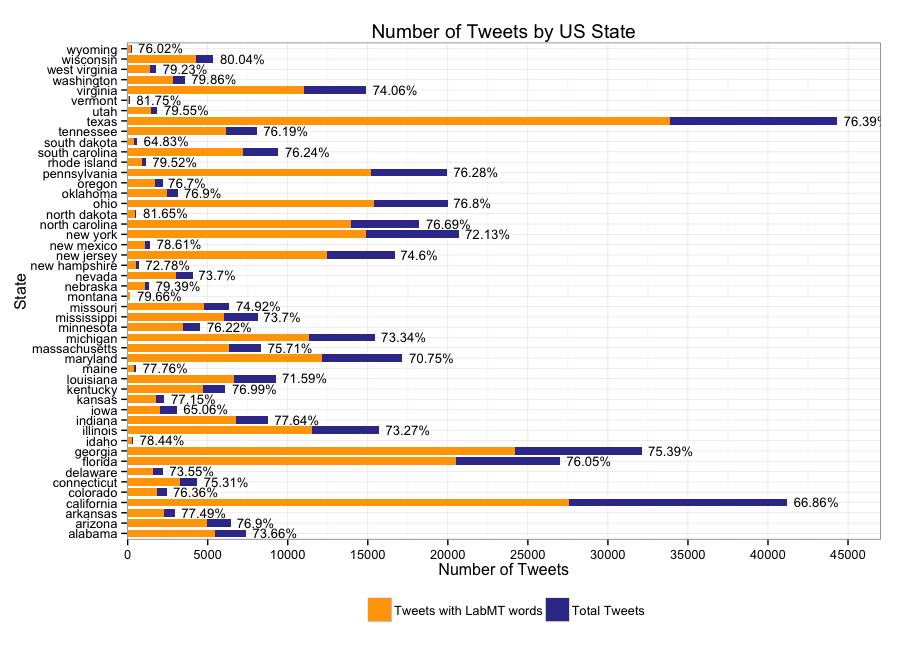
\includegraphics[width=\textwidth]{images/tweets_by_state}
\caption{Stacked bar chart for the number of tweets by US state. In blue the total number of tweets, and in orange the number of tweets with words from the LabMT corpus of words. In front of each bar we have the percentage of tweets that have LabMT words.}
\label{fig:tweets_by_state}
\end{figure}

Finally we will be using the 2012 Gallup-Healthways Well-being Index results \cite{GallupHealthway2013} \footnote{available at http://info.healthways.com/wbi2013}. This study has an \emph{Overall Well-Being Index} that we will use as a hapiness index to correlate with our results.

\section{Methodology}
\subsection{LabMT Tweet Processing}
As stated in \ref{sec:datasets}, to measure sentiment (hereafter happiness) in the areas from the corpus of words collected, we use the Language Assessment by Mechanical Turk (LabMT) word list \cite{Dodds2011}. This word list has a total of roughly 10'000 of individual words, which have been scored on a scale of 1 (sad) to 9 (happy), resulting in a measure of average happiness for each given word \cite{Kloumann2012}. For a given text T containing N unique words, we calculate the average happiness $h_{avg}$ by:
\begin{align*}
h_{avg}(T) = \frac{\sum_{i=1}^{N} h_{avg}(w_i)f_i}{\sum_{i=1}^{N} f_i} \tag{1}\label{eq:1}
\end{align*}
where $f_i$ is the frequency of the $i$th word $w_i$ in $T$ for which we have a happiness value $h_{avg}(w)$, and $p_i = f_i/\sum_{i=1}^{N}f_i$ is the normalized frequency of word $w_i$. This is a similar approach of the original ANEW research \cite{Bradley1999}, that's explained in \cite{Dodds2009}.
This method makes no attempt to take the context of words or the meaning of a text into account. While this might lead to difficulties in accurately determining the emotional content of small texts, it was proved that for sufficiently large texts this approach nonetheless gives reliable (if eventually improvable) results \cite{Dodds2011,Mitchell2013,Dodds2009,Kloumann2012}.
Following Dodds et al. \cite{Dodds2011}, we remove all words $w_i$ for which the happiness score falls in the range $4 < h_{avg}(w_i) < 6$ when calculating $h_avg(T)$. Removal of these neutral words has been demonstrated to provide a suitable balance between sensitivity and robustness in \cite{Dodds2011}. Following \cite{Mitchell2013}, to avoid the problem that some states have happier names than others we removed (a) each state name from the calculation for $h_{avg}$; and (b) all variants of the racial pejorative or ‘N-word’, since variants of this word have very low happiness values, and consequently were found to be highly influential in determining the state happiness score, however upon examining individual tweets \cite{Mitchell2013} found that this word appeared to be being used in conversation as a more colloquial stand in for the word `friend', and not in fact in any particularly negative sense, therefore the word was unfairly biasing \cite{Mitchell2013} the results towards the negative and removed it.

To increase the amount of tweets considered in the study, we also processed the same sample using a Spanish list of words resulting from work by \cite{Redondo2007} \footnote{word list available at http://link.springer.com/article/10.3758\%2FBF03193031}. To avoid duplication of tweets that have words in both lists, we only consider the word list that have more word matches with a tweet. This process allowed us to increase our number of tweets in near 40'000.


\subsection{Geolocating Tweets}
Each geotagged tweet from the data set was processed in order to extract its latitude and longitude coordinates, searching for those fields in the Twitter API \footnote{available at https://dev.twitter.com/docs/platform-objects/tweets}. After stripping those two fields, and to be able to match each tweet to a US state, we used the \emph{sp} R package \footnote{available at http://cran.r-project.org/web/packages/sp/} more specifically the \emph{over} function, which does consistent spatial overlay for points, grids and polygons, i.e., if a latitude/longitude point $x$ and a polygon $P$ representing a state is given, the over function returns \emph{true} or \emph{false}, if that point is inside the polygon - if a certain tweets belongs to a certain state.


\subsection{Gallup-Healthway Score}
We will correlate our happiness results with with the 2012 Gallup-Healthways Well-being Index \cite{GallupHealthway2013} \footnote{available at http://info.healthways.com/wbi2013}. Since LabMT score goes from 1 to 9, we had to rescale the Gallup-Healthways Overall Well-Being Index from a percentage scale (0-100) to the LabMT. For this we used the known `typical' function to rescale values from one range to another:
\begin{align*}
rescale_(x) = \frac{(b-a)(x-min)}{max-min} + a \tag{2}\label{eq:2}
\end{align*}
where, for our case: $min = 0$, $max = 100$, $a = 1$ and $b = 9$.


\subsection{Score by US State}
After having all tweet associated with a state, we had to choose on of the three statistics that allowed us to get a score for a whole state state, using either the \emph{mean}, \emph{median} or the \emph{mode}. To choose between them we plotted the histograms for the score distributions of some states (see Fig. \ref{fig:tweets_distribution}), to observe the patterns for tweet distribution, and we calculated the correlation factor between those three statistics and the Gallup-Healthway Index.

\begin{figure}[!ht]
\centering
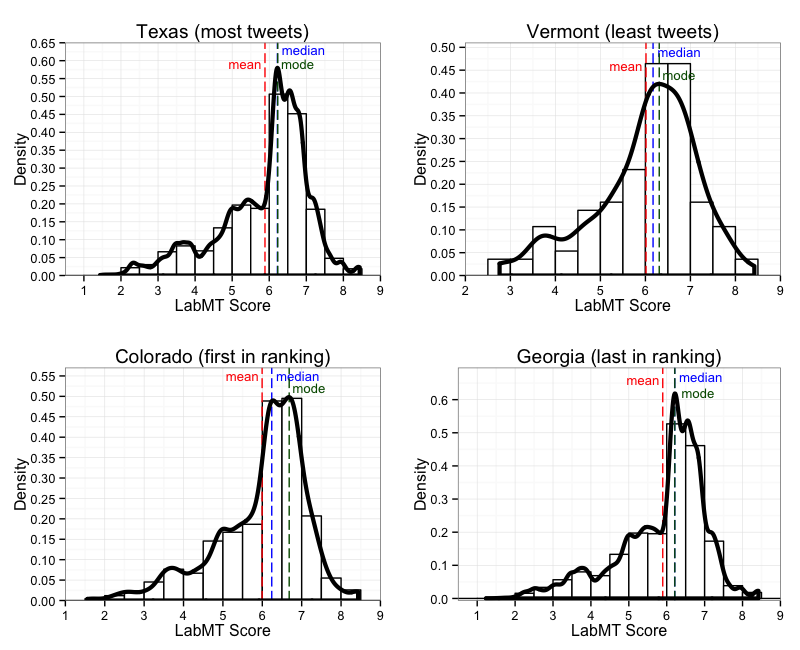
\includegraphics[width=\textwidth]{images/tweets_distribution}
\caption{Histograms and density lines for Texas (state with most tweets), Vermont (state with least tweets), Colorado (first in state happiness ranking) and Georgia (last in happiness state ranking). Vertical red line is the mean of the scores, vertical blue line is the median of the scores, and vertical green line is the mode of the density function for the scores.}
\label{fig:tweets_distribution}
\end{figure}

An initial analysis lead us to choose the \emph{mode} because the correlation was the highest, and after that decision we decided to use the mode of the density function to improve even more our correlation score. We limited its interval to $[1,9]$, the range of values of the LabMT word scores, and used a adjust (smooth) factor of 0.80. This allowed us to achieve a correlation of approximately $0.45$, which indicates an average correlation coefficient between between the LabMT score mode and the Gallup-Healthway Well-Being score. The correlation results are shown below:
\begin{flalign*}
    & X = \textrm{Gallup-Healthway Well-Being Index score by state} \tag{3}\label{eq:3}\\
    & cor(X , Y) = 0.187 ,\textrm{ with Y = mean of LabMT tweet scores by state} \\
    & cor(X , W) = 0.029 ,\textrm{ with W = median of LabMT tweet scores by state} \\
    & cor(X , Z) = 0.448 ,\textrm{ with Z = mode of LabMT tweet scores by state}
\end{flalign*}


\subsection{Visualization}
Finally we present our results using one of the visualization methods discussed in \cite{Nollenburg2007}, which is also used in \cite{Mitchell2013,Dodds2011}, the Choropleth map.
Th Choropleth map uses the graphic variables describing properties of color or texture to show properties of non-overlapping areas, such as provinces, districts, or other units of territory division. A number of categories is mapped to distinct colors or textures which are used to fill the areas accordingly. For the colors used on our choropleths, we used the \emph{RdYlGn} palette from the \emph{RColorBrewer} R package \footnote{available at http://cran.r-project.org/web/packages/RColorBrewer/}, which has a set of default color palettes based on the work done by \cite{Harrower2003} \footnote{available at http://colorbrewer.org}. We presented our maps using the \emph{globular projection} detailed in \cite{Bolstad2012}.

\section{Results}
First we plot the average happiness of all US Continental States (all states except Alaska and Hawaii) in Fig. \ref{fig:scores_by_state}. In this chart we plot our results redefining the scale so we get a greater amount of different colors near the mean value of our state scores. This way we avoid using an uniform scale, that causes most of the states to be with the same color. Our scale is an approximation of a Normal Distribution, but in a ad-hoc manner: $scale = \langle min, mean - (sd/2), mean - (sd/3) , mean, mean + (sd/3), mean + (sd/2), max \rangle$. The result is a scale that increases the amount of different colors near the mean, and uses the same ones in the extremities.

\begin{figure}[!ht]
\centering
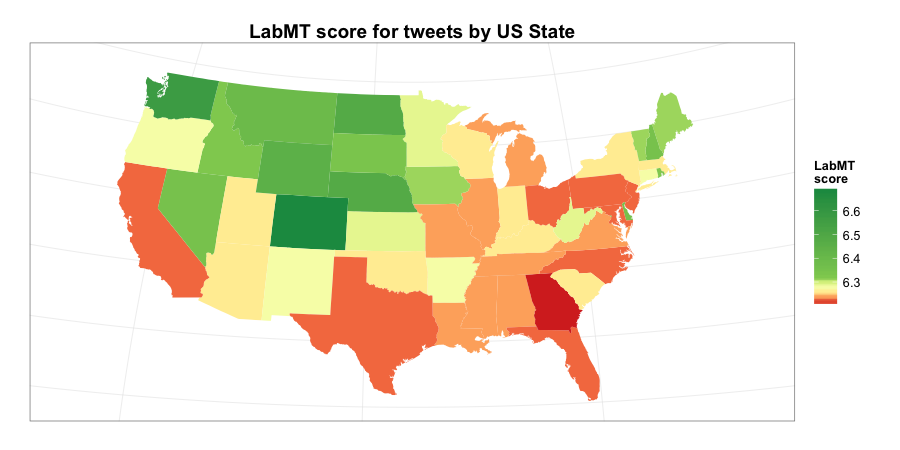
\includegraphics[width=\textwidth]{images/scores_by_state}
\caption{Choropleth showing \emph{mode} word happiness for geotagged tweets in all Continental US states collected during the calendar year 2012. The happiest 5 states, in order, are: Colorado, Washington, Nebraska, North Dakota, Wyoming. The saddest 5 states, in order, are: Georgia, Texas, Pennsylvania, Ohio, North Carolina. The full state ranking is shown in Appendix section.}
\label{fig:scores_by_state}
\end{figure}

At such a coarse resolution there is little variation between states, which almost all lie between 0.09 - which is the sd (standard deviation) for the $h_{avg}$ - of the mean value for the entire United States of $h_{avg} = 6.30$. The exception are the top 5 states which are in average 0.23 above the mean value. The happiest state is Colorado with a score of $h_{avg} = 6.68$ and the saddest state is Georgia with a score of $h_{avg} = 6.21$. The striking observation that we take from the ranking is the high correlation between the state's position in the ranking and the number of tweets of that state, $cor(\textrm{number of tweets}, \textrm{ranking}) = 0.77$, and also a high correlation between the score and the number of tweets, $cor(\textrm{number of tweets}, \textrm{LabMT score}) = -0.48$. This means that the more tweets a state has the lower it will be in the ranking (and the sadder it will appear to be). In fact, if we split our states into equal parts (6 states each group), we can clearly see the average number of tweets per group increases as we lower in the ranking (see Table X).

\begin{table}[h]
\centering
\begin{tabular}{>{\centering\arraybackslash}m{1in}  >{\centering\arraybackslash}m{1in}}
\toprule
Ranking    & Average number of tweets \\
\midrule
1-12th     & 1376                     \\
13-24th    & 4391                     \\
25-36th    & 5344                     \\
37-48th    & 14479                    \\
\bottomrule
\end{tabular}
\linebreak
\caption{Average of tweets per position in state ranking}
\label{tab:tab1}
\end{table}

Another interesting way to look at the data is to emulate the style that Gallup-Healthway uses for the choropleth in their report. They split up the scores per state in five quintiles, coloring them in the map. For the sake of easier comparison, we present both the original and our own choroplet using the same scheme Gallup-Healthway uses.

\begin{figure}[!ht]
\begin{subfigure}[b]{\textwidth}
\centering
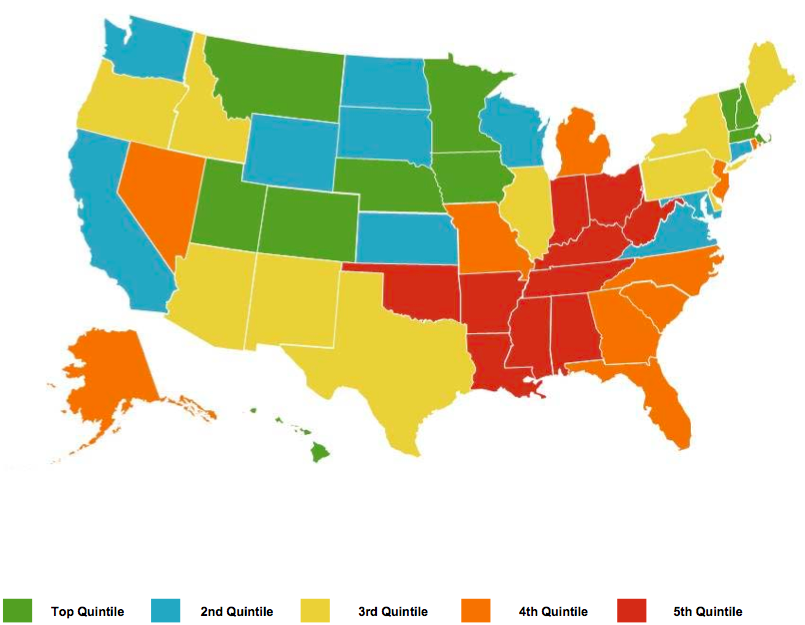
\includegraphics[width=\textwidth]{images/gallup_2012}
\end{subfigure}
\begin{subfigure}[b]{\textwidth}
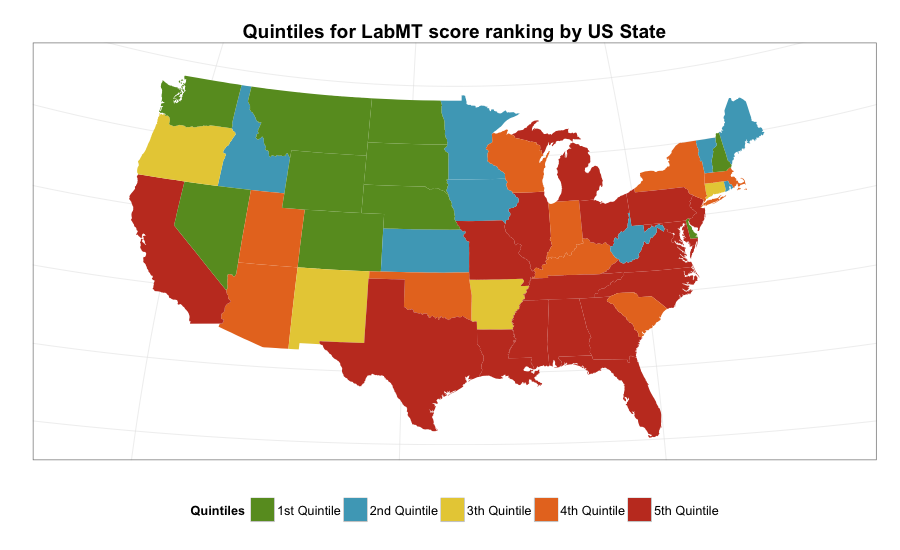
\includegraphics[width=\textwidth]{images/scores_by_state_gallup_style}
\end{subfigure}
\caption{Gallup-Healthway Well-Being Index choropleth vs Our own choropleth using the same quintile schema as well as the same color code.The happiest 5 states for Gallup-Healthway study are, in order, are: Colorado, Minnesota, Utah, Vermont, Nebraska. The saddest 5 states, in order, are: Arizona, Tennessee, Mississippi, Kentucky, West Virginia. The full state ranking is shown in Appendix section. Source \cite{GallupHealthway2013}}
\label{fig:gallup_vs_labmt}
\end{figure}


Even tough there is no striking resemblance between the two charts, if you take into account the little variation of the scores that we discussed before, we can assume that a state could easily be on another quintile (except the top 5, as we also discussed before). In the Southeast we have similar results, with some of the states that should be in the 4th Quintile are in the 5th. Northeast section is very far apart with many of the values on the 4th/5th Quintile when they should be in the 3rd/2nd, still in the north part there's some improvement. Midwest section has yet again some striking resemblance between the 1st and 2nd Quintile states. Southwest state also have some resemblance with some states switching between the 3rd and 5th Quintile. Finally, the West appears similar with some states switching between the 1st and 2nd Quintile, but with a staggering difference in California. In fact, there are very few states that jump more than 3 Quintiles in their classification.

You can attest that analyzing the ranking differences in the bump chart in Fig. \ref{fig:bump_chart} that compares the changes in ranking between the LabMT approach and Gallup-Healthway score. What we aim with this graph is a high number of straight (or almost straight) lines. Those indicate that the rank stayed the same (or almost the same) in both approaches. As we expected (since we achieved a correlation of approximately $0.45$), a reasonable amount of lines are straight. Regarding the lines that aren't straight, we can observe that they connect extremes of the ranking (with rare exceptions).

\begin{figure}[!ht]
\centering
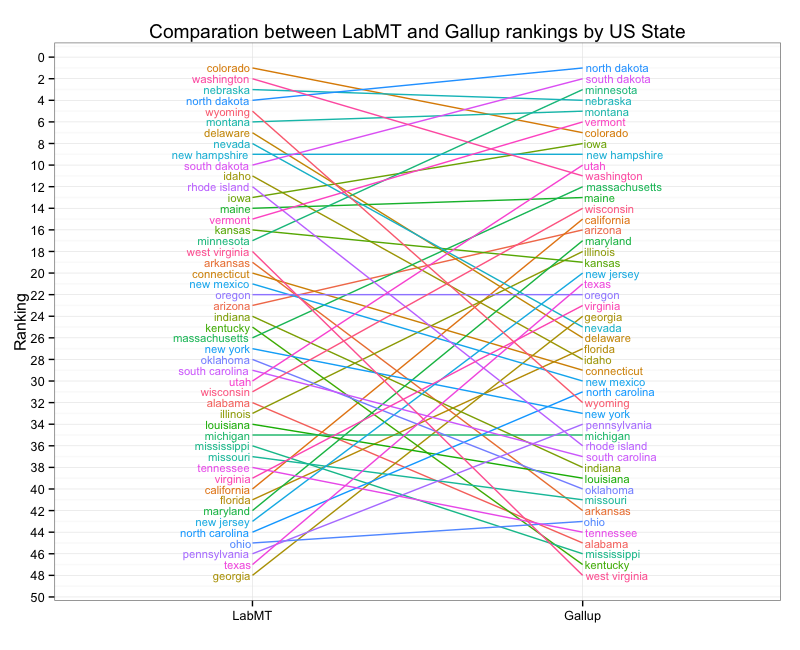
\includegraphics[width=\textwidth]{images/bump_chart}
\caption{Bump chart that compares the changes in ranking between the LabMT approach and Gallup-Healthway score. On the right column you have the ranking from our approach using LabMT word list. On the left column we have the Gallup-Healthway ranking for the calendar year of 2012 \cite{GallupHealthway2013}, minus the states that we didn't considered in our study, i.e., Alaska and Hawaii.}
\label{fig:bump_chart}
\end{figure}

\begin{figure}[!ht]
\centering
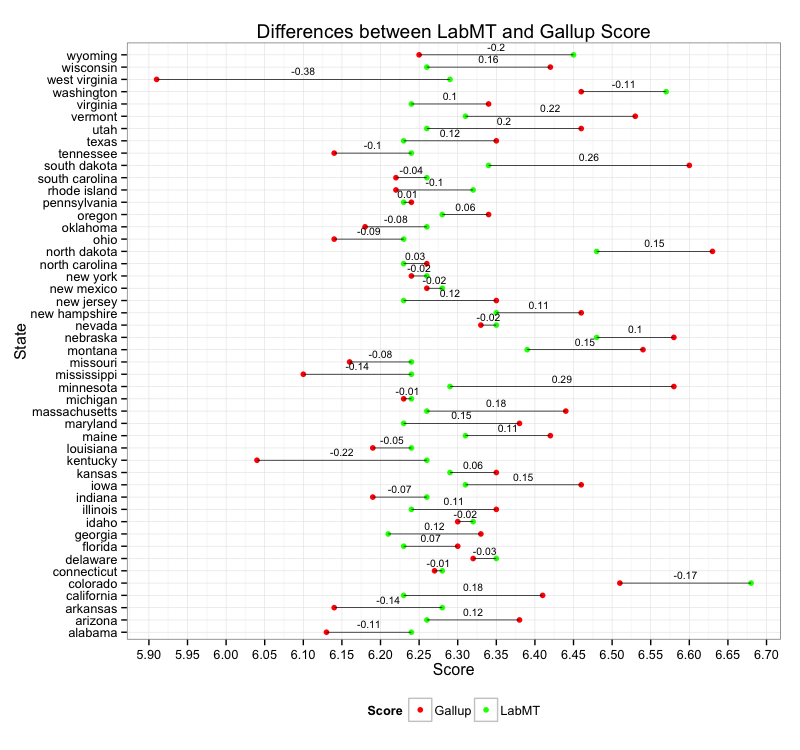
\includegraphics[width=\textwidth]{images/differences}
\caption{Difference in the score using our LabMT approach, and Gallup-Healthway Well-Being Index, rescaled to the range used in \cite{Dodds2009,Dodds2011} method, i.e. 1 to 9. We can see - just like it happen with the ranking - that when the difference is small, it is very small, and when the difference is large, it's significantly large.}
\label{fig:differences}
\end{figure}

Regarding score difference in spite of the little variation there is our scores, the average difference between Gallup-Healthway score and is just 0.02. What happens is that, and we can verify that analyzing Fig. \ref{fig:differences}, we either have very small differences (in the range of few hundredths) or we have very large differences (in the range of several tenths). This leads to situations we can see in Fig. \ref{fig:bump_chart}, where many times we see a state changing very few positions in ranking and other times changing many positions.

Finally, and showing the potential of our dataset, we make the same choroplet as we did in Fig. \ref{fig:scores_by_county}, but instead of states we show US Counties. The scale is the same as in the original choroplet so the comparison between the two maps is easier. This forced us to cap the values used in the county map to the minimum and maximum score values that we found in the state map.
There is a great amount of dispersion regarding the number of tweets by county, with a mean of 230 tweets per county but with a sd of 675. That's why we observe weird patterns like the state of California, where the counties are mainly green but the red counties are the ones with the most tweets. When we move to a coarser scale, those counties with the highest number of tweets will contribute more towards the mode score, leading to a shift in the overall state score.

\begin{figure}[!ht]
\centering
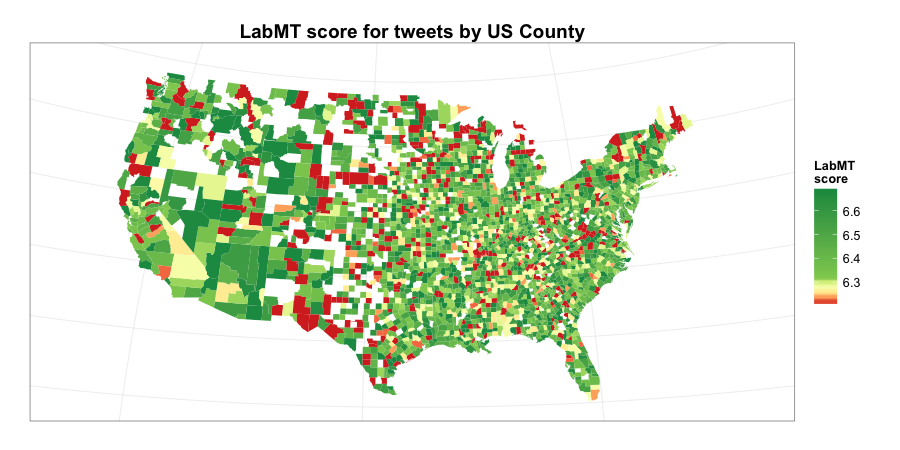
\includegraphics[width=\textwidth]{images/scores_by_county}
\caption{Choropleth showing \emph{mode} word happiness for geotagged tweets in all Continental US counties collected during the calendar year 2012. The scale is the same as the one used in Fig. \ref{fig:scores_by_state}, with values capped to the range of scores of the state.}
\label{fig:scores_by_county}
\end{figure}

\section{Discussion and Future Work}
In this paper we have examined word use in urban areas in the United States, using a simple mathematical method which has been shown to have great flexibility, sensitivity and robustness. We have used this tool to map areas of high and low happiness and score individual states (and also counties) for average word happiness.

A FALAR
CORRELACOES COM OUTROS ESTUDOS
- Falar da correlação com o outro paper
- falar da correlacao do outro paper com o gallup
- falar da correlacao entre gallup e este
CORRELACOES ENTRE NUMERO DE TWEETS E FELICIDADE
CONCLUIR FALANDO DA ROBUSTEZ DO MODELO


There are a number of legitimate concerns to be raised about how well the Twitter data set can be said to represent the happiness of the greater population. Roughly 15\% of online adults regularly use Twitter, and 18-29 year-olds and minorities tend to be more highly represented on Twitter than in the general population \cite{Smith2012}. Furthermore, the fact that we collected sample is small compared with the overall Twitter usages, and that the geotagged tweets are even less means that our data set is a non-uniform subsample of statements made by a non-representative portion of the population. One could improve the amount of geotagged tweets, considering for the non-geotagged tweets that they were made from the city the user filled in its Twitter registration form.

In this work we have only scratched the surface of what is possible using this particular dataset. We have not examined whether or not these methods have any predictive power—future research could look at how observed changes in the Twitter data set, predict changes in the underlying social and economic characteristics measured using traditional census methods.

FALAR DE UM POSSIVEL MODELO REGRESSAO UTILIZANDO O NUMERO DE TWEETS, ALGO QUE NAO FOI FEITO

% References
\bibliographystyle{splncs03}
\bibliography{remote}

\end{document}
